\section{Context \& Motivations}

\def\UrlFont{\bfseries}

\begin{frame}{Spirals Team}
    \center
    
\includegraphics[width=0.5\textwidth]{figures/spirals}
    \vspace{7mm}

    \large{Spirals is conducting research activities in the domains of distributed systems and software engineering.}
    \vspace{7mm}
    \begin{itemize}
        \centering
	    \item[] \textbf{PowerAPI}
        \item[] \textbf{Spoon}
        \item[] \textbf{APISENSE}
    \end{itemize}
\end{frame}

\begin{frame}{APISENSE}
    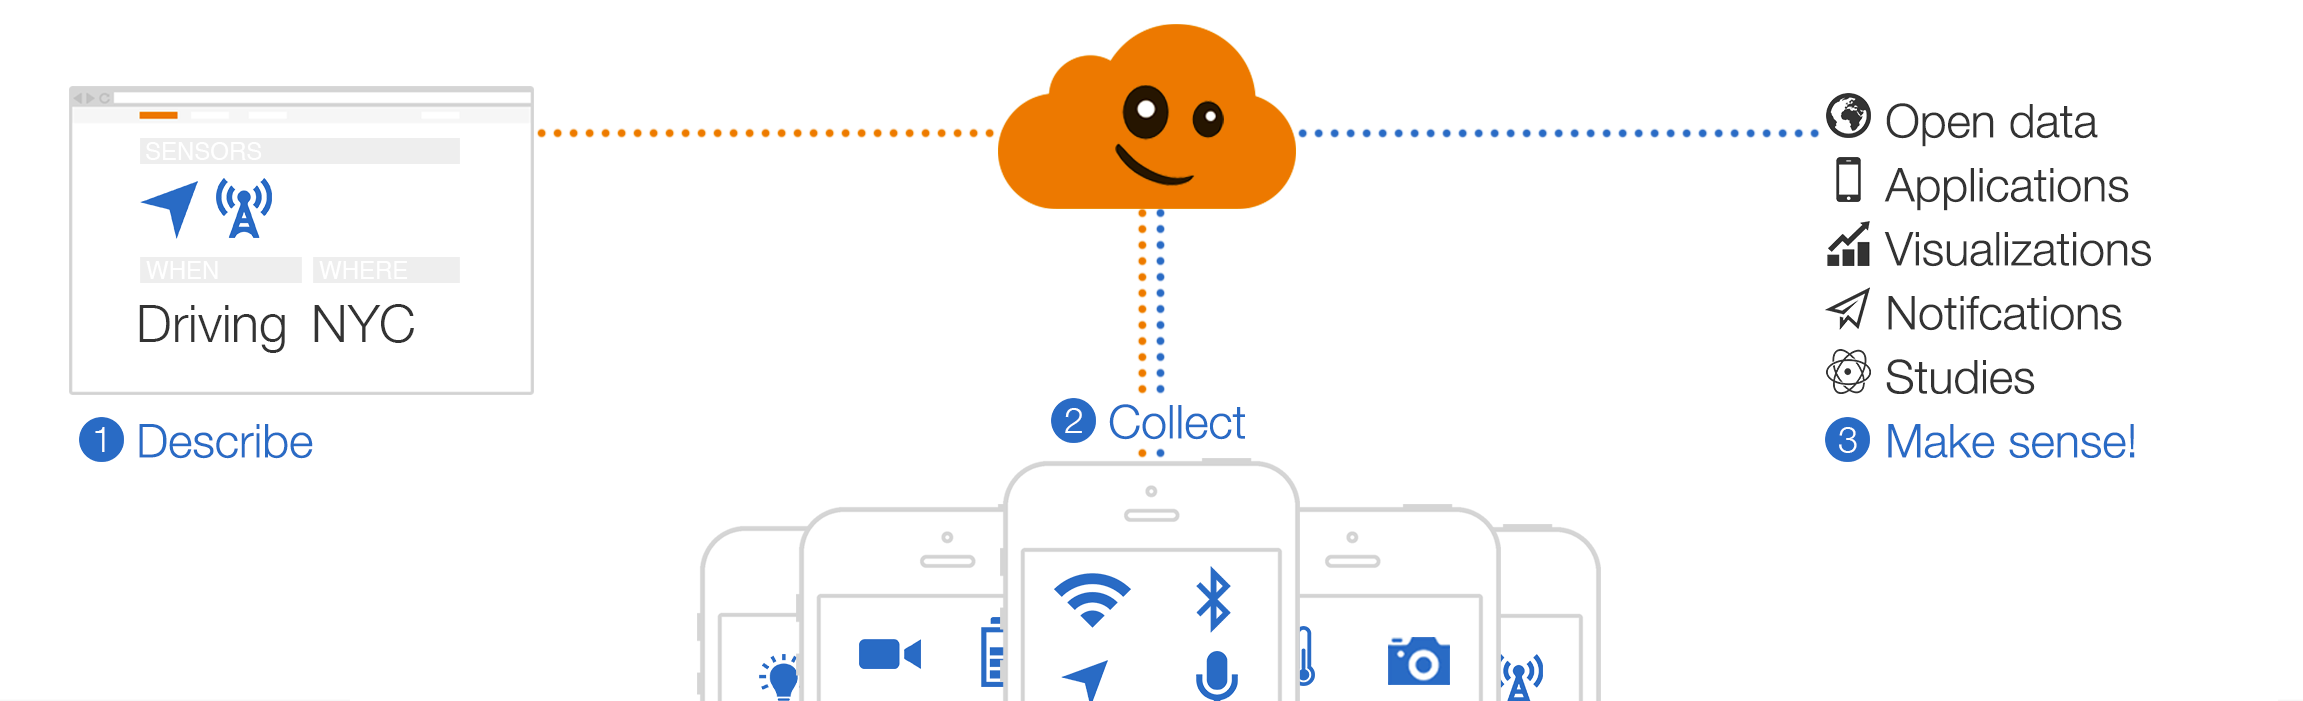
\includegraphics[width=\textwidth]{figures/apisense}
    \center
    \vspace{7mm}
    
    \url{https://apisense.io}
\end{frame}

\begin{frame}{Threats}
    \center
    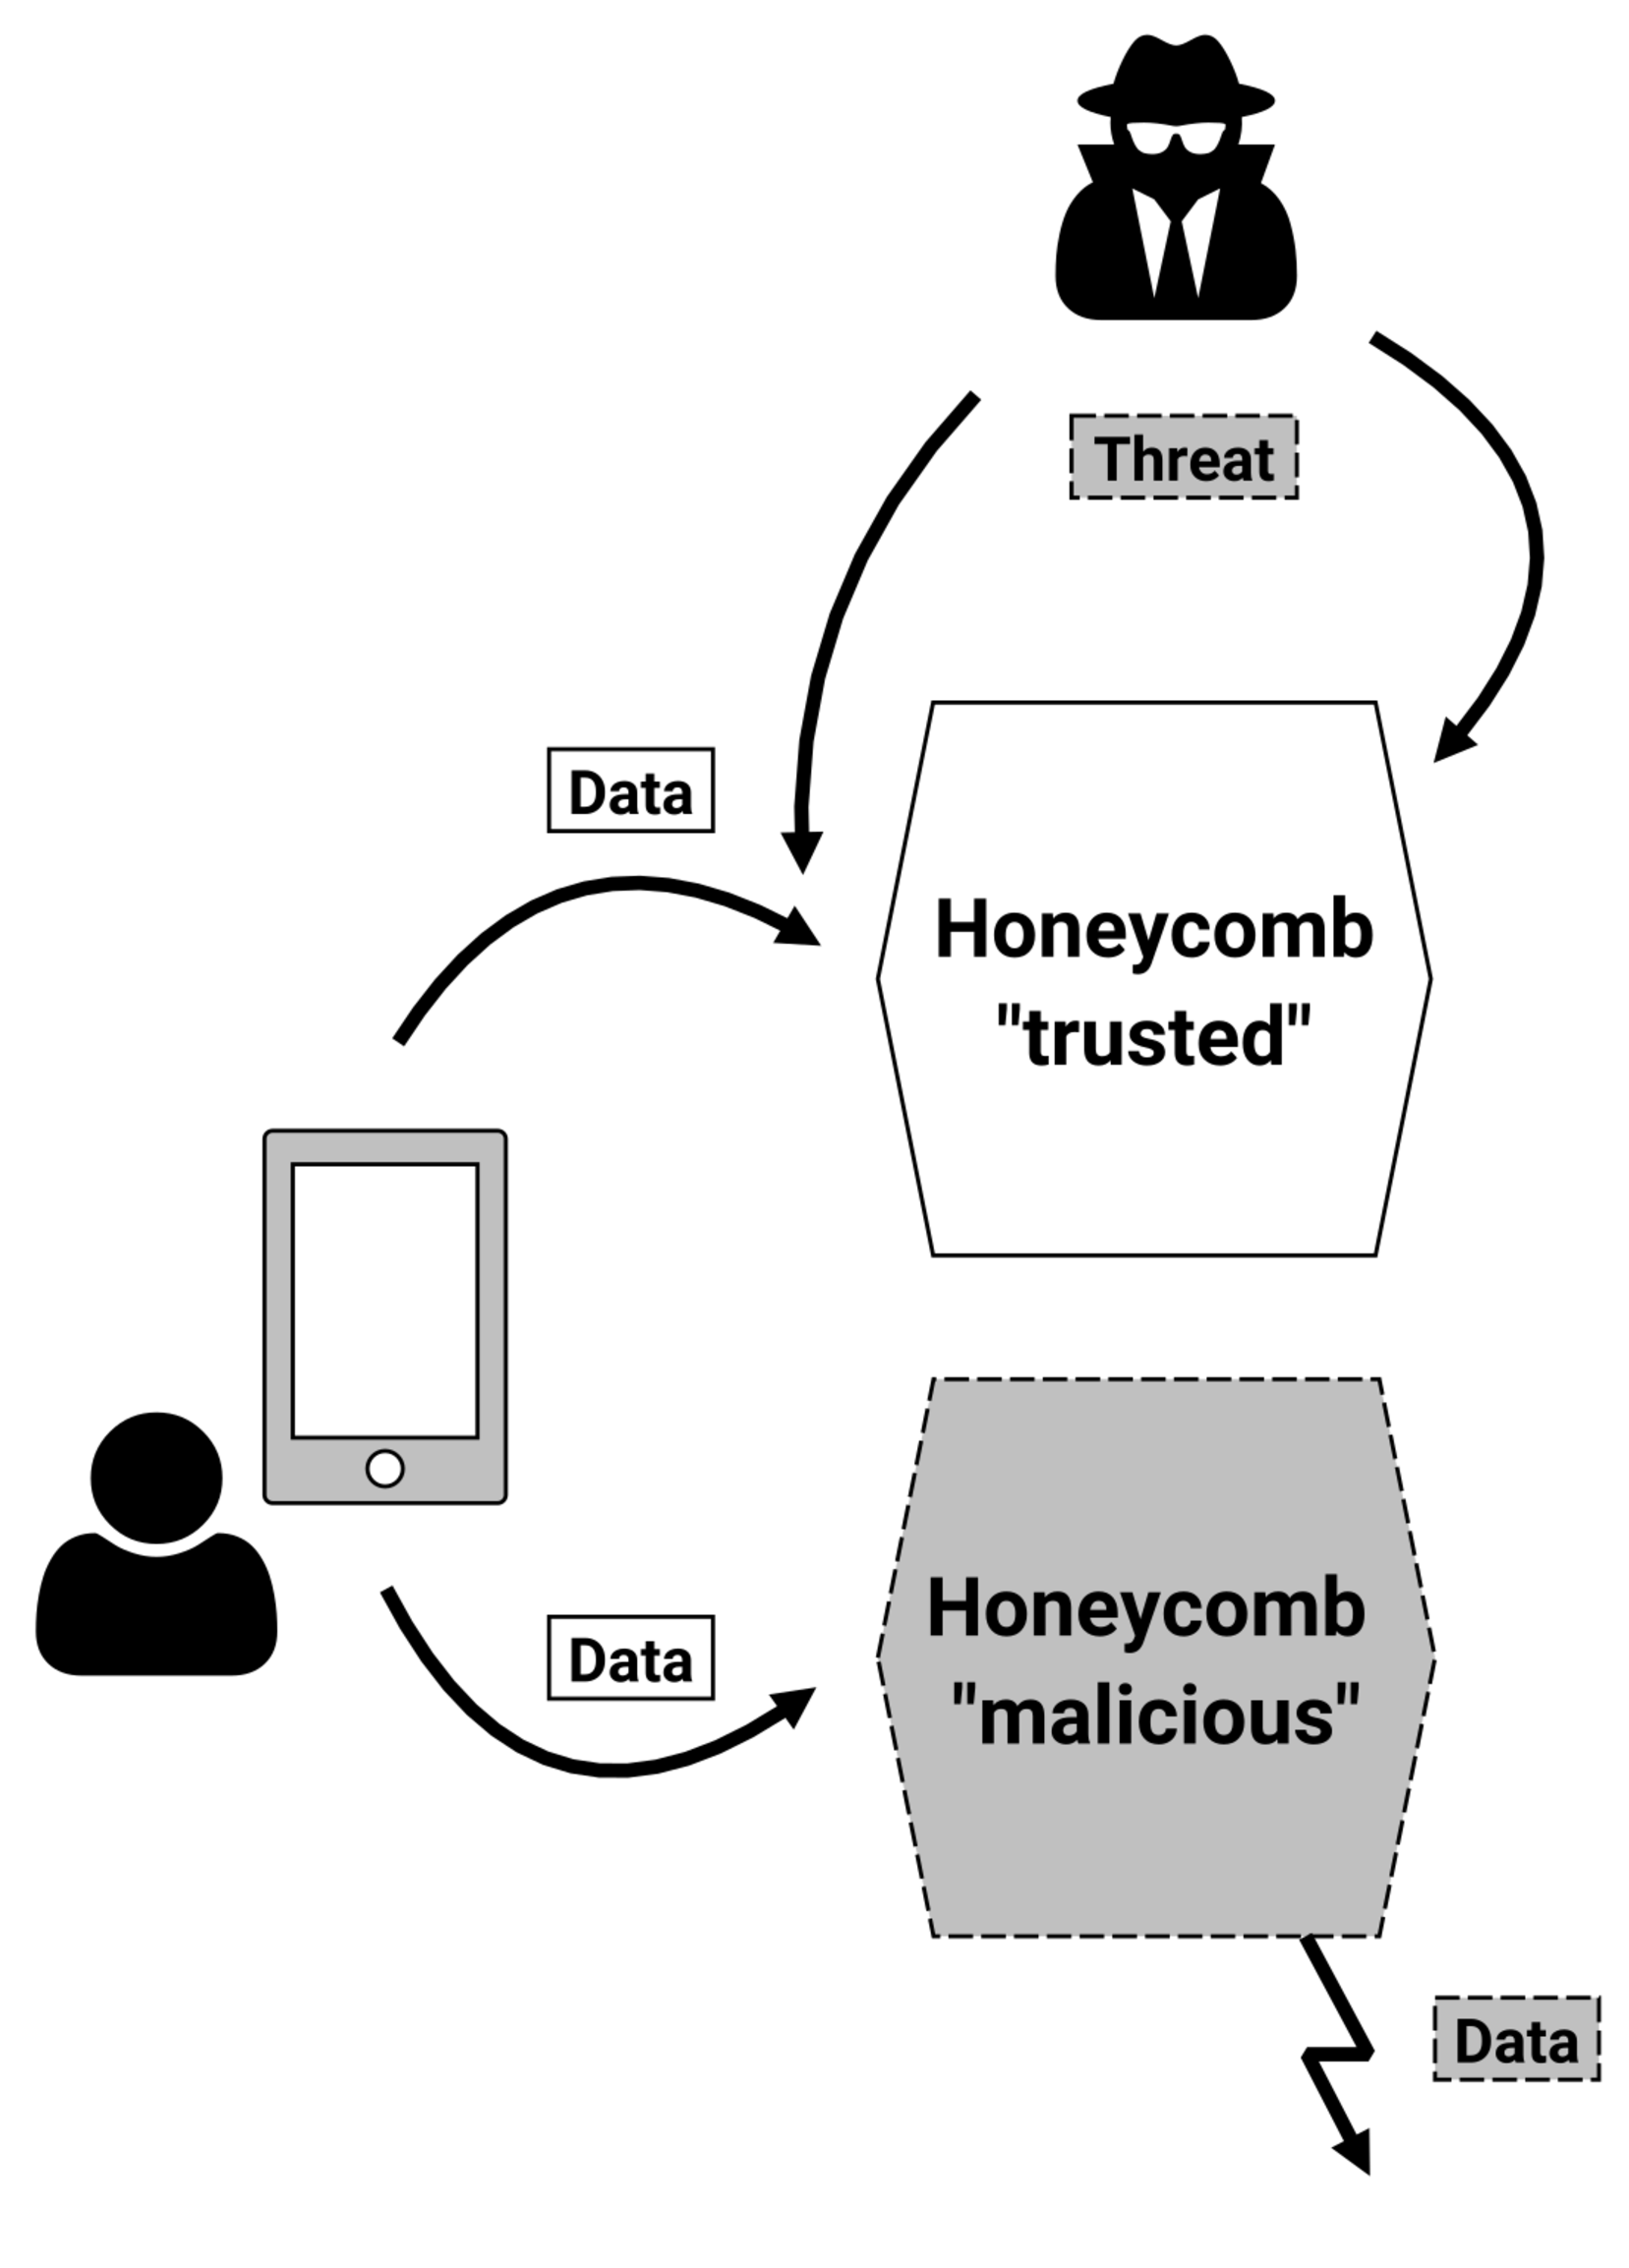
\includegraphics[width=0.5\textwidth]{figures/threat}
\end{frame}

\begin{frame}{IP Linkage}
    \begin{figure}[<+->]
        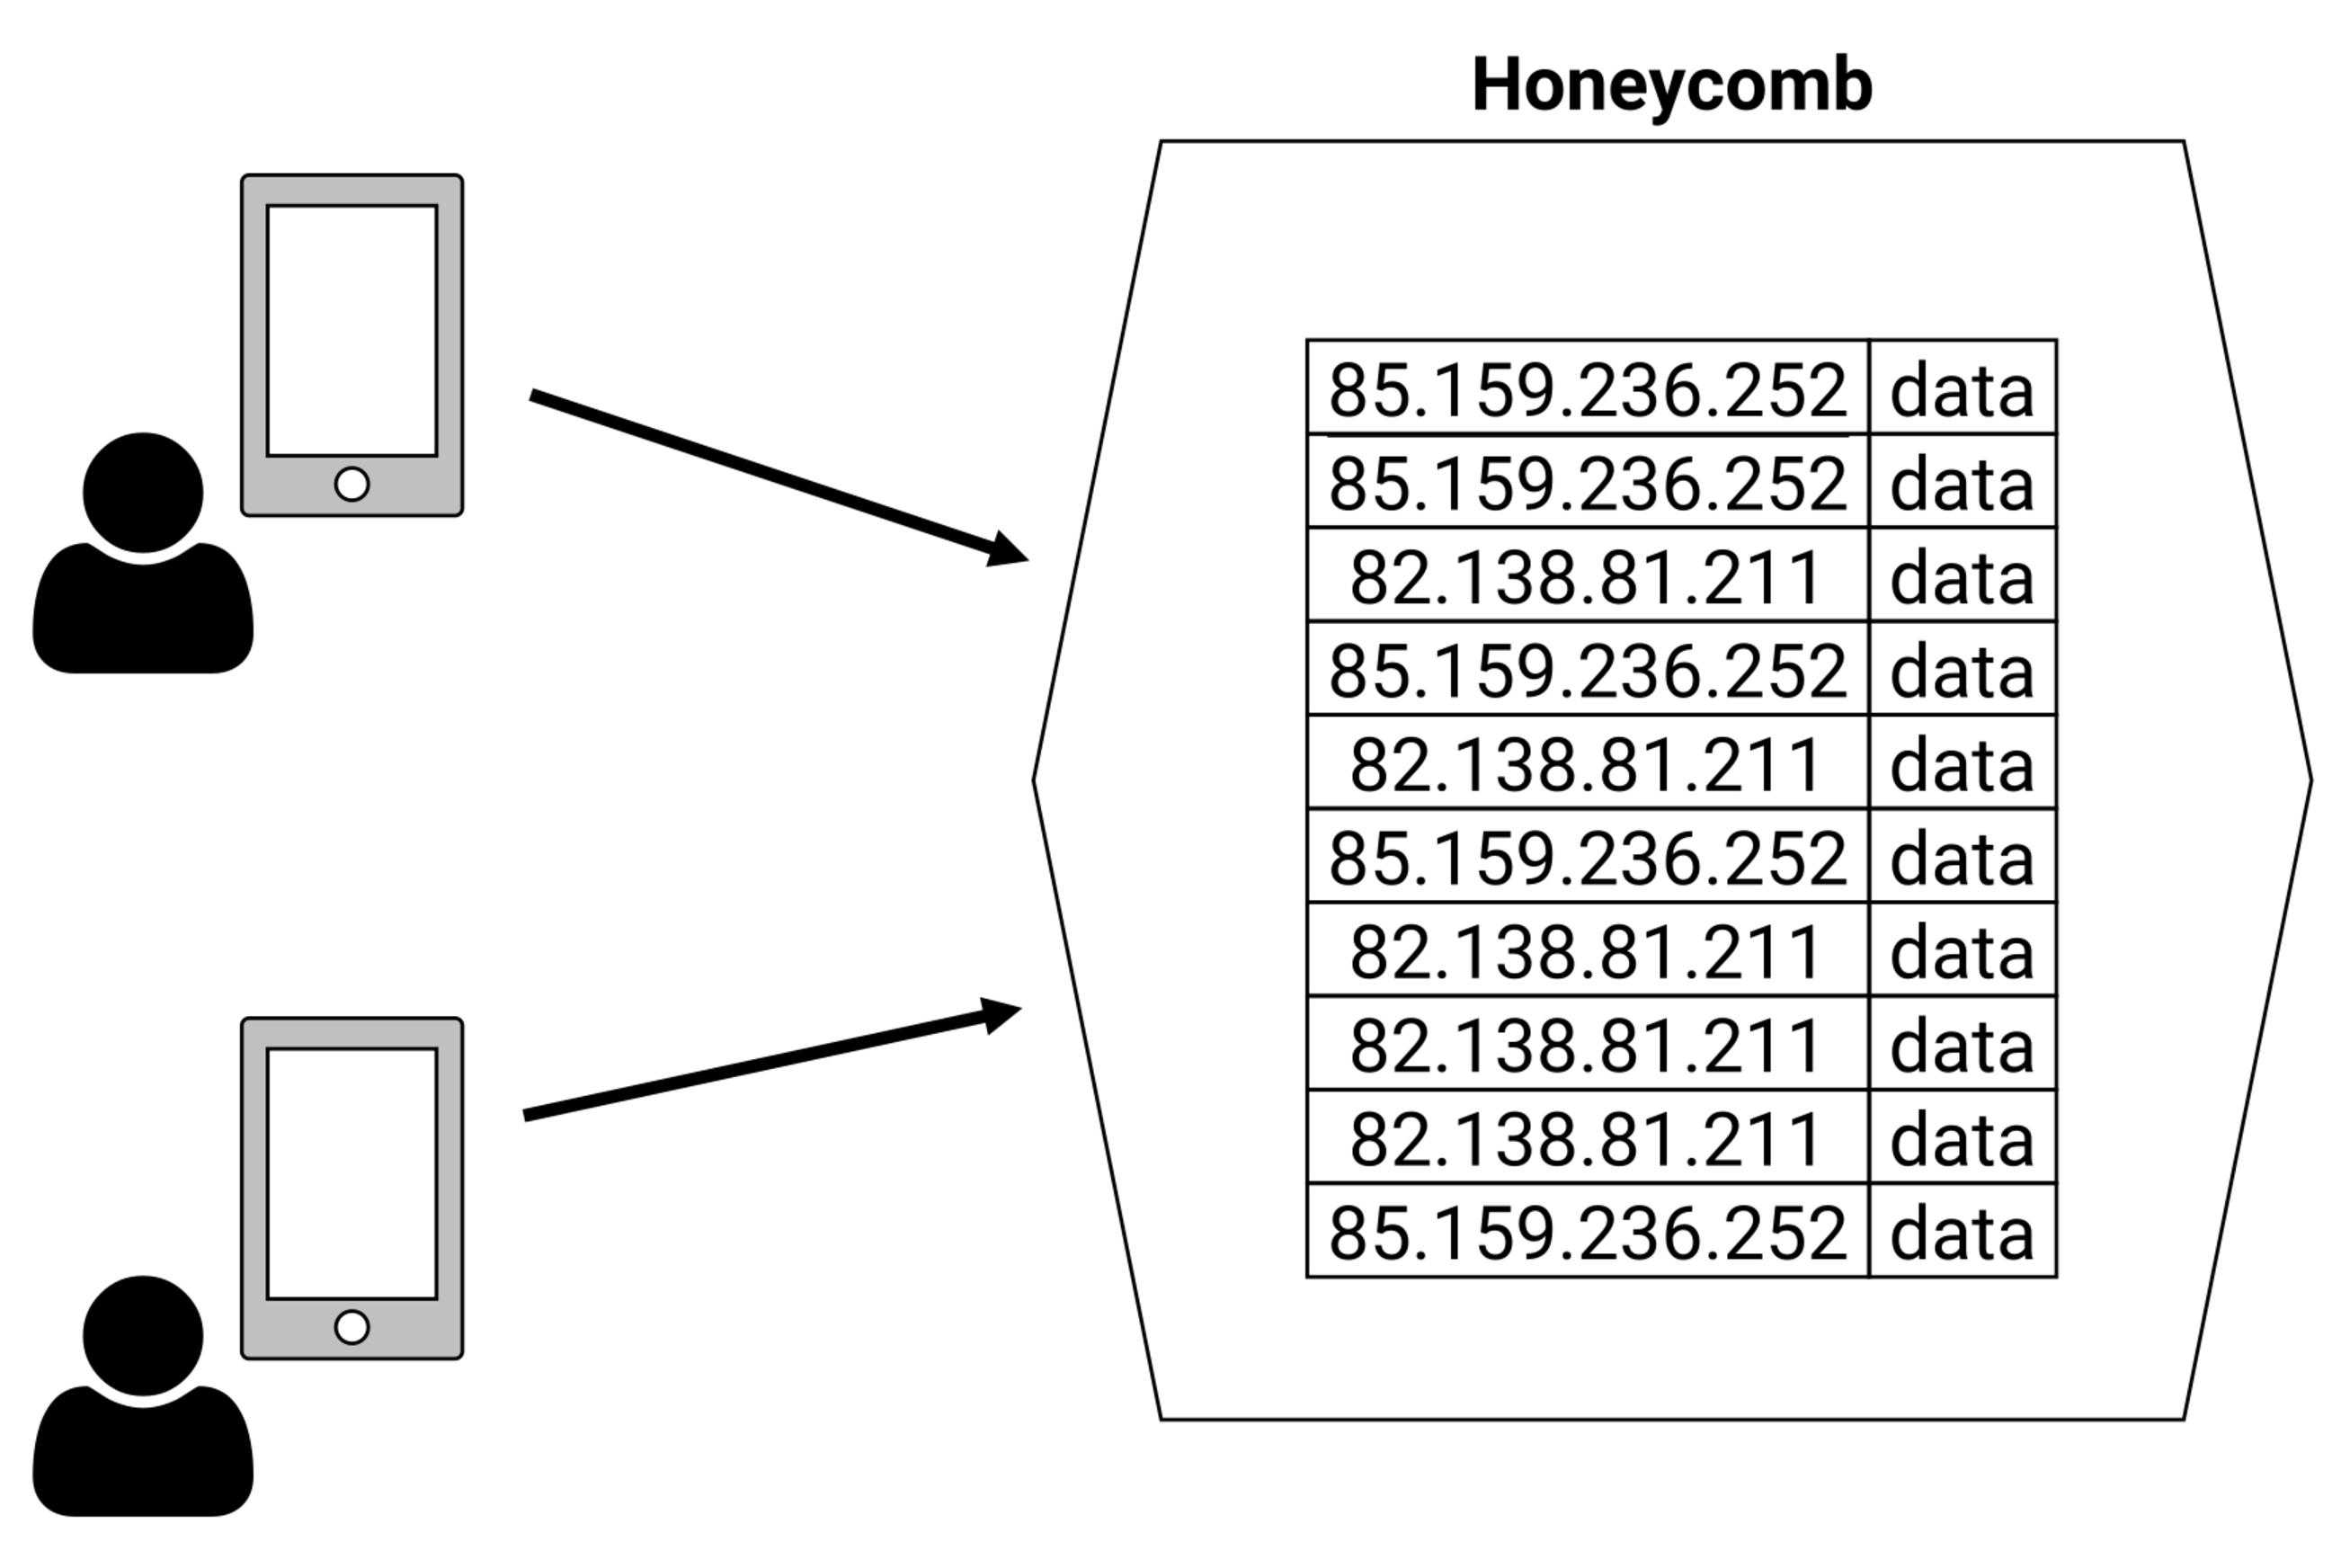
\includegraphics[width=\textwidth]{figures/ip}<1>
        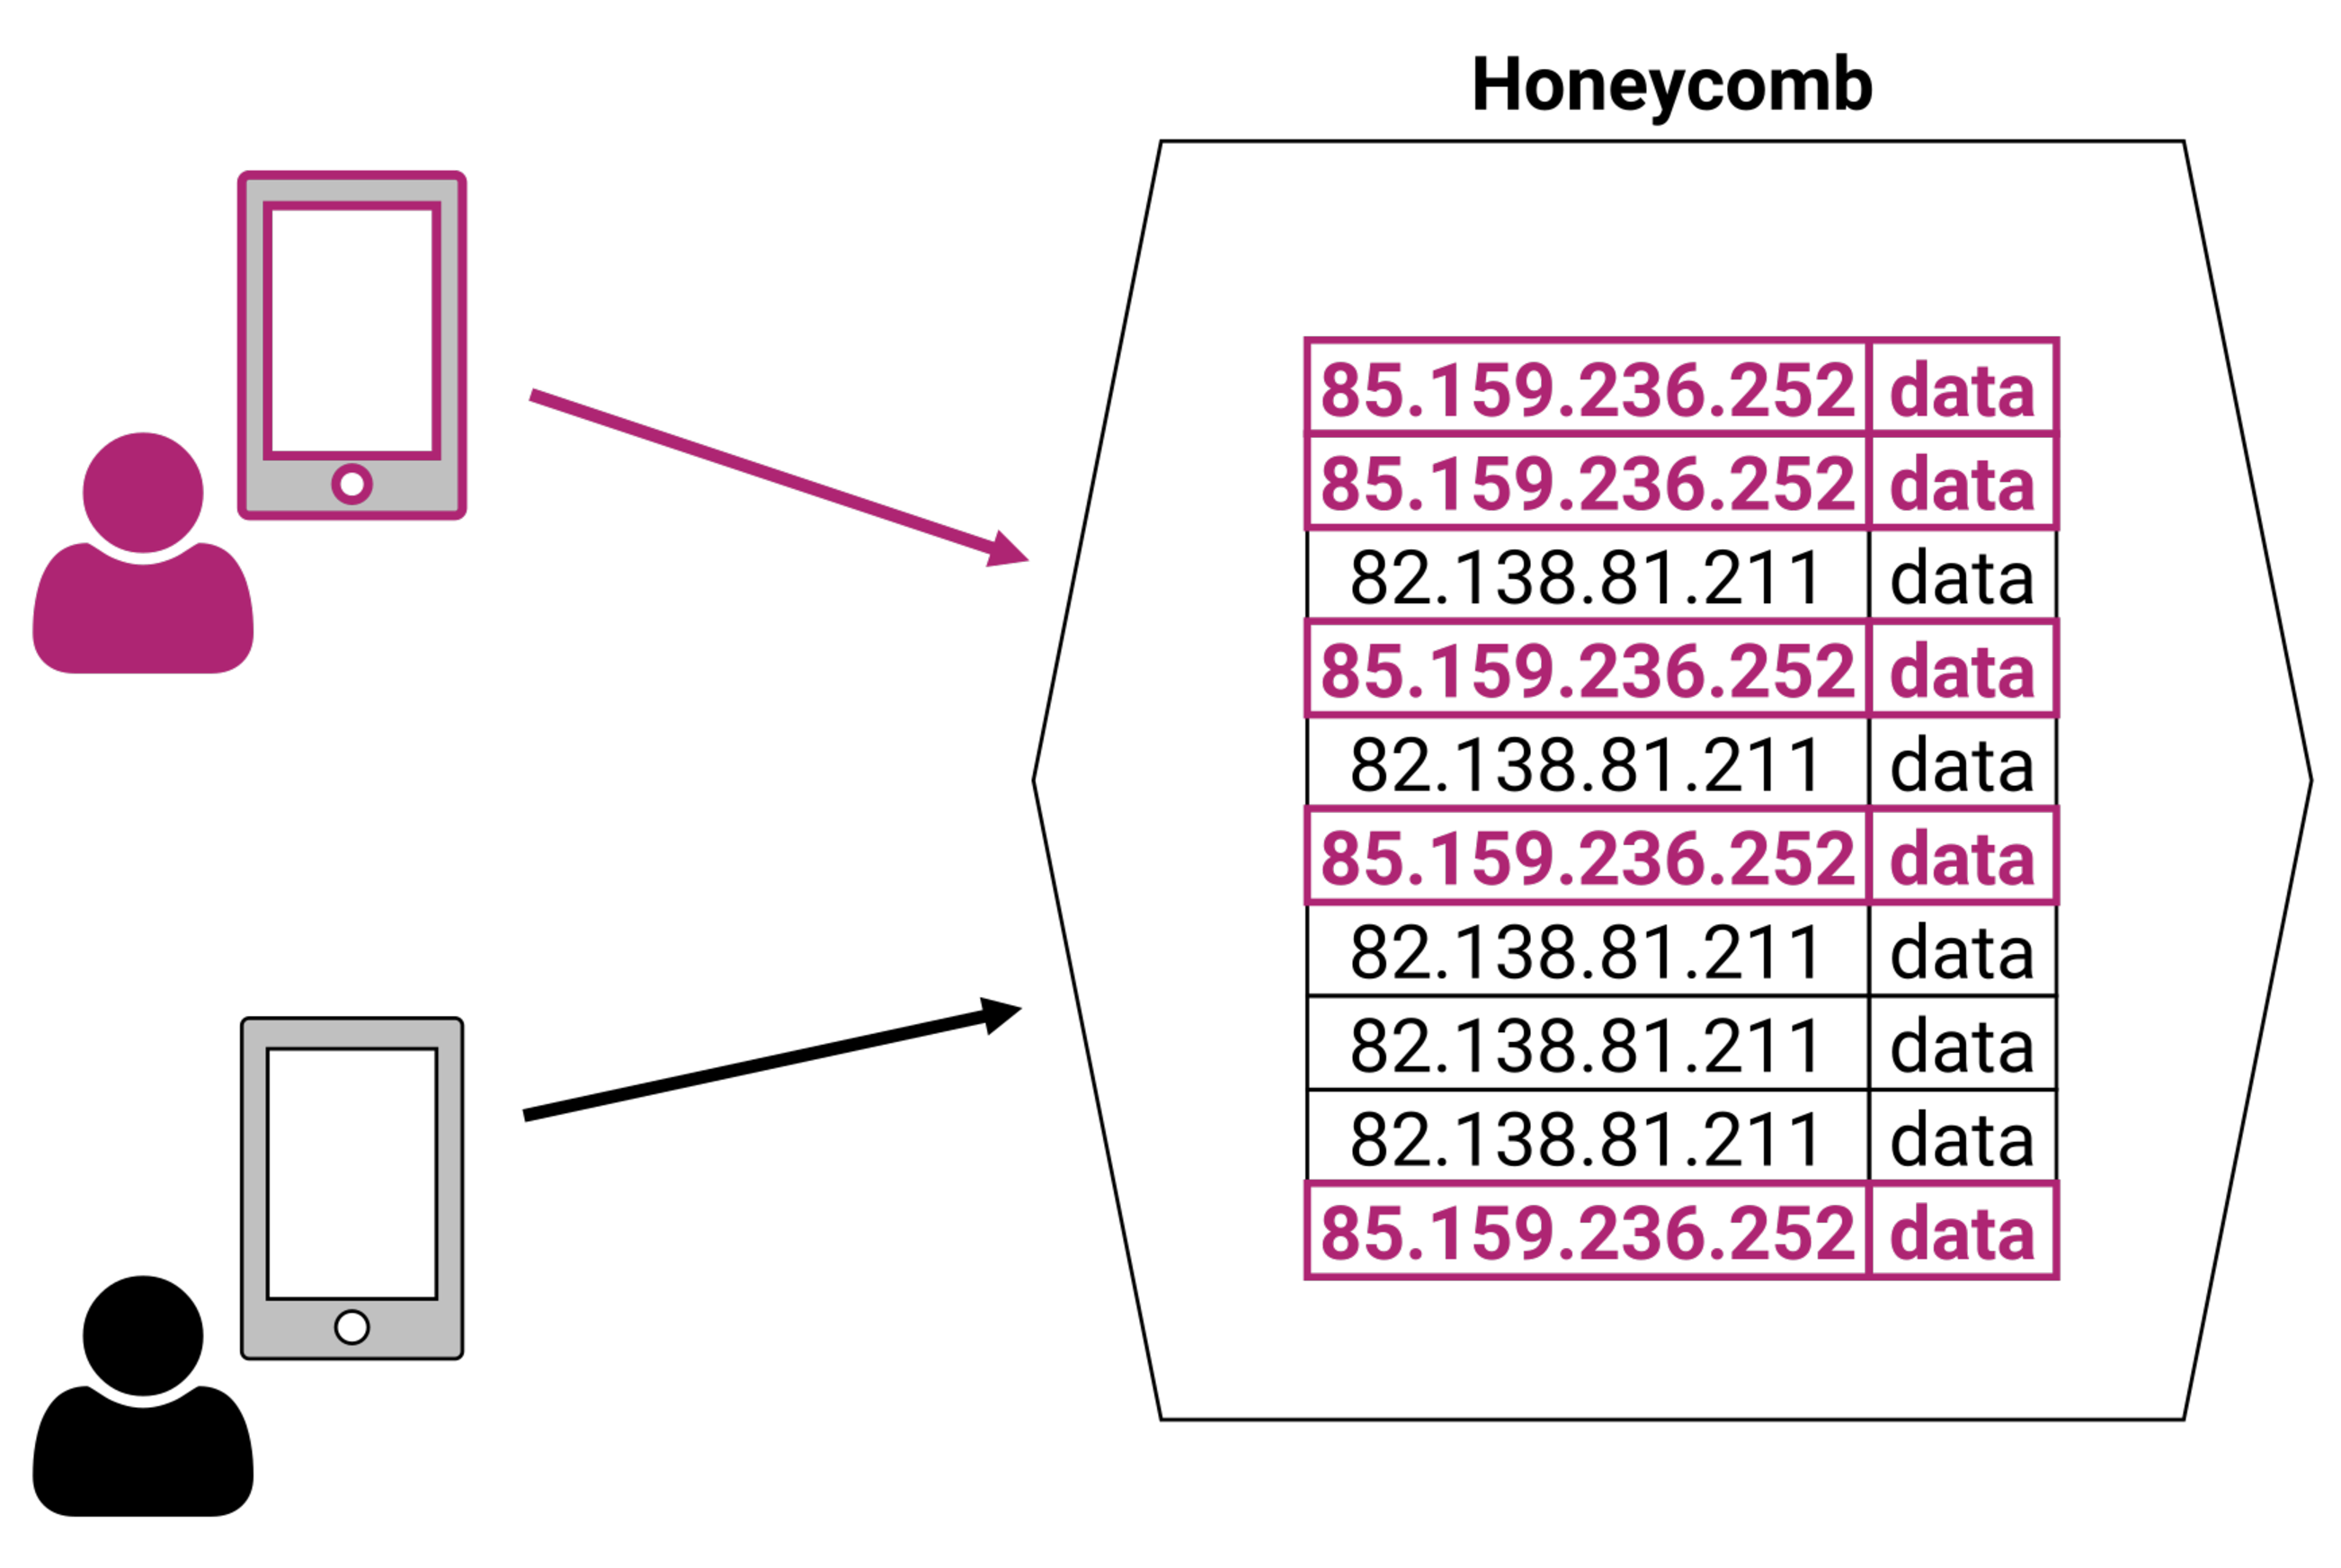
\includegraphics[width=\textwidth]{figures/ip1}<2>
        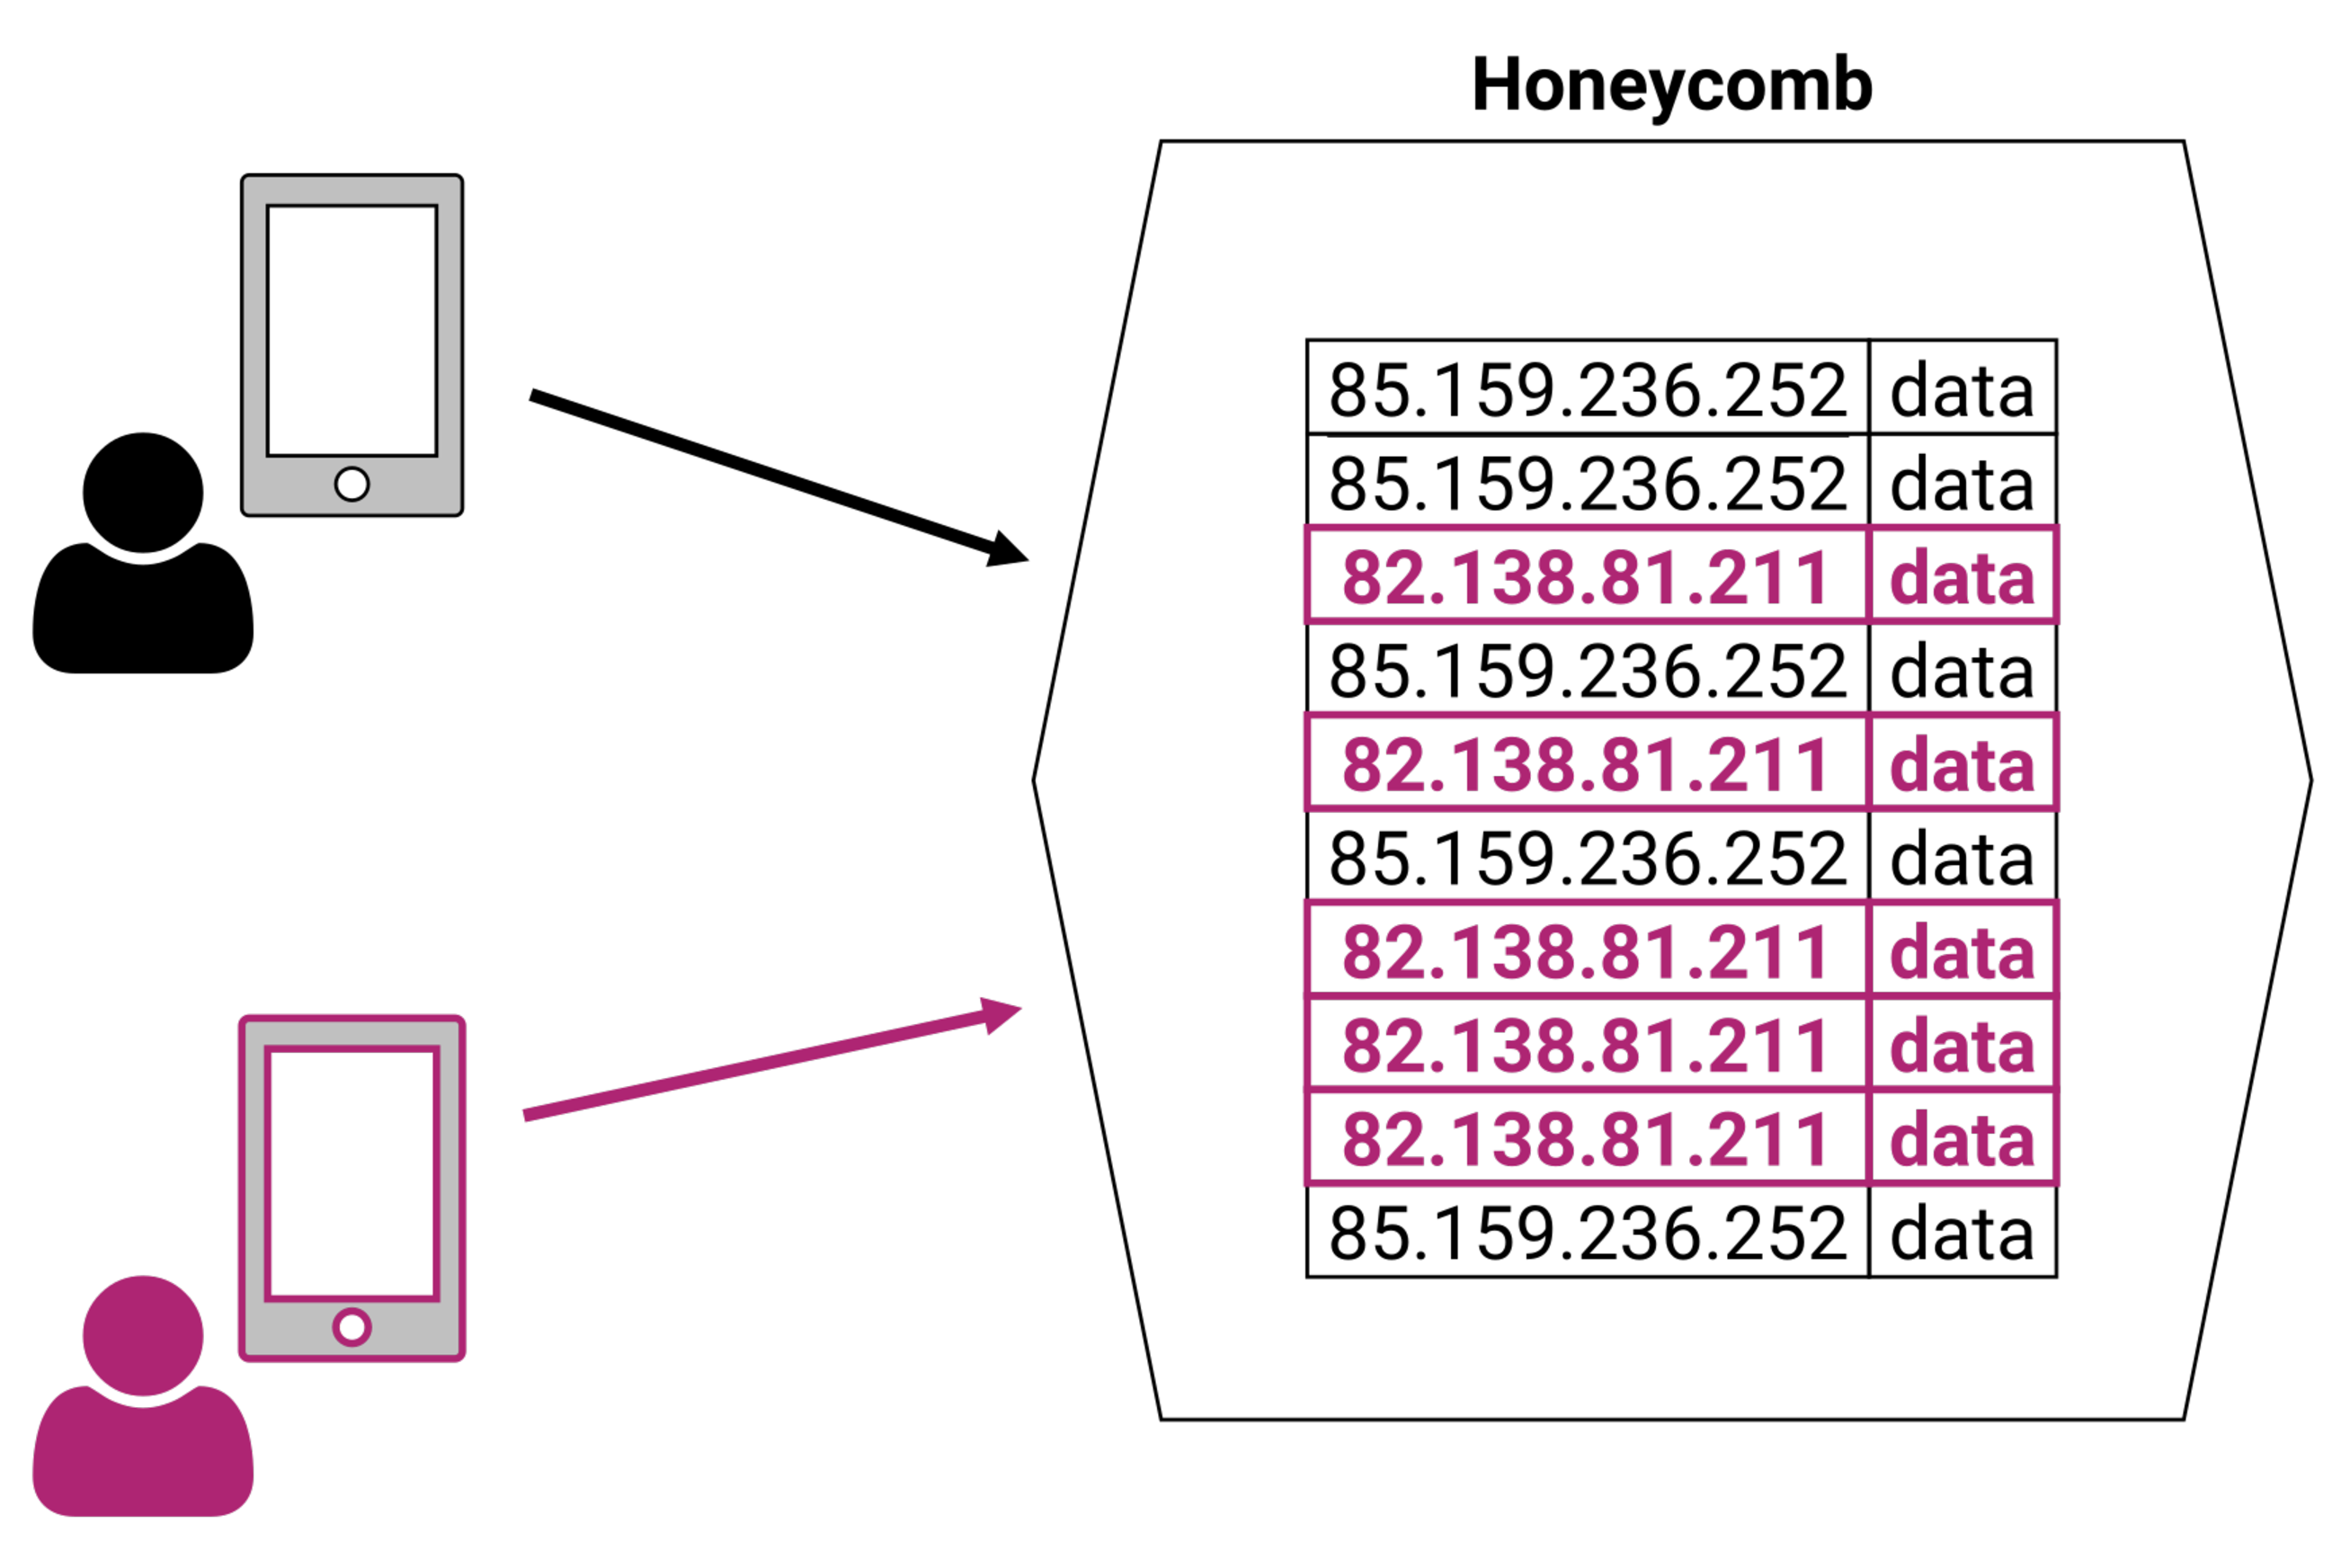
\includegraphics[width=\textwidth]{figures/ip2}<3>
    \end{figure}
\end{frame}

\begin{frame}{Goal}
    \LARGE{Define a method that \textit{scrambles} the data \textbf{before} sending their to the end-server.}
\end{frame}

\begin{frame}{Proposals}
    \begin{itemize}
	    \item \textbf{Foug\`ere}, a \textit{data dissemination} library that uses a \textit{distance} notion to disseminate data.
	    \item \textbf{AndroFleet}, a \textit{large-scale emulation platform} for the Android OS. 
    \end{itemize} 
\end{frame}